\documentclass{mgragh} % opcje: robocza,man
\usepackage[cp1250]{inputenc}  % opcja latin2 dla Linuxa lub cp1250 dla Windows
\usepackage[polish]{babel}
\usepackage[OT4]{fontenc}
\usepackage{polski}
%%
%%
\makeindex 
% \includeonly{Mgr_pom,Mgr_wst,Mgr_roz1,Mgr_roz2,Mgr_lit}

\bibliographystyle{ddabbrv}
%\nocite{*}

\begin{document}
%%
%%
%% ======== METRYCZKA PRACY ========
\title{O budyniu tyczkowym}
\author{Nikodem Jura}
\author{Krzysztof Rajda}
\promotor{dr hab. in� Marek Kisiel-Dorohinicki}
\nralbumu{11957}
\uczelniaNazwa{Akademia G�rniczo-Hutnicza}
\uczelniaImienia{im. Stanis�awa Staszica}
\wydzial{Elektroniki, Automatyki, Informatyki i Elektrotechniki}
\kierunek{Informatyka}
\specjalnosc{Skr�canie d�ugopis�w}
\rok{2006}

\maketitle
%%
\slowakluczowe{maciejka, nafta, serek}

%\keywords{a,b,c,d,e,f,g,h} 
%%
%%
%% ======== NASZE MAKRA ========
%%

%----------------- nasze definicje -----------------% 
\newtheorem{stw}{\indent Stwierdzenie}[chapter]
%------------------------------%
\newcommand{\id}[1]{\index{#1}}  
\newcommand{\wi}[1]{#1\index{#1}}  
\newcommand{\wwi}[1]{\emph{#1}\index{#1}}  
\newcommand{\mwi}[1]{\textbf{#1}\index{#1}}
\newcommand{\ii}[1]{\textit{#1}}
%\newcommand{}{}

%---------------------------------------------------%



%%
%% ======== SPIS TRE�CI ========
%%
\tableofcontents
%%
%% ======== STRESZCZENIE PRACY (POLSKIE) ========
\begin{streszczenie}
%%

%--------------------------------------------------------------------%

%%
\end{streszczenie}
%%
%% ======== G��WNA CZʌ� PRACY ========
%%
%% ==== WST�P ====
%%
\begin{wstep}
%%
\section{Wprowadzenie}
%\subsection{Machine learning}
%\subsection{Indukcyjne bazy danych}
%\subsection{Zastosowania}

Integracja technologii baz danych z nowoczesnymi metodami indukcyjnego
generowania wiedzy wydaje si� dawa� istotne korzy�ci w perspektywie
budowy system�w wspomaganie decyzji. Systemy nazywane czasem
indukcyjnymi bazami danych potrafi� odpowiedzie� nie tylko na pytania,
dla kt�rych odpowied� znajduje si� w bazie danych, ale r�wnie� na
pytania, kt�re wymagaj� zsyntetyzowania i zastosowania wiarygodnej
wiedzy, wygenerowanej przez indukcyjne wnioskowanie z fakt�w z bazy
danych i wcze�niejszej wiedzy.  Indukcyjne bazy danych mog� by�
postrzegane jako naturalny krok w rozwoju system�w bazodanowych \cite{bib3}.

\begin{figure}[ht]
    \centering
        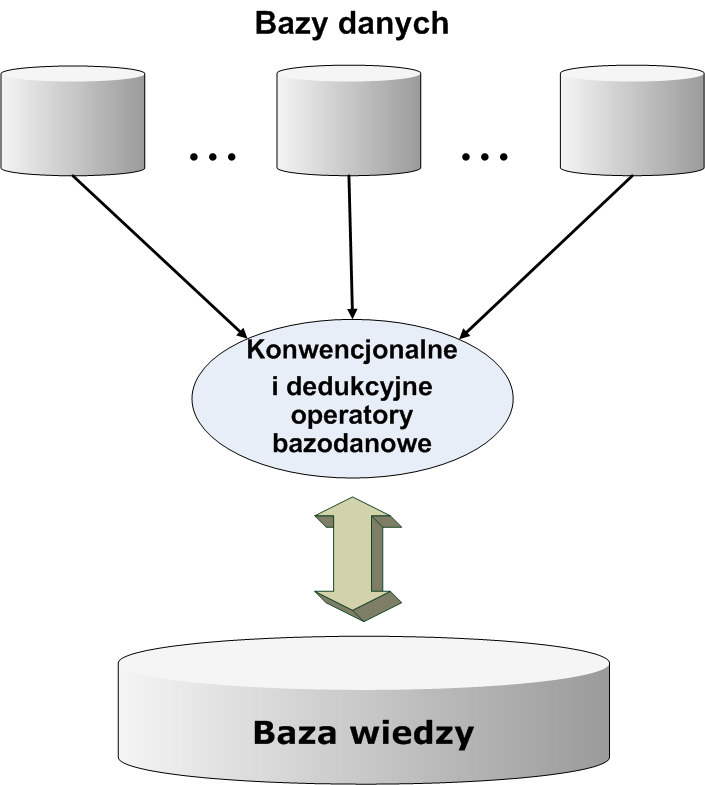
\includegraphics[width=0.70\textwidth]{img/knowledge_mining.png}
    \caption{Indukcyjne bazdy danych}
    \label{fig:architecture}
\end{figure}

\bigskip
W pracy przedstawiona zostanie architektura i wybrane aspekty
implementacji platformy \emph{Salomon}, jak r�wnie� zaprezentowane
zostan� mo�liwo�ci jego wykorzystania na przyk�adzie wybranych
algorytm�w pozyskiwania wiedzy z danych.

%\newpage
%%
\end{wstep}
%%
%% ==== ROZDZIA� 1 ====
%%
%% A tutaj tak dla przyk�adu jest \part
\part{Musztarda kotwiczna}

\chapter{Wprowadzenie do przypraw walcowych}
%%
% \input{Mgr_roz1}
%%
\mgrclosechapter
%%
%% ==== ROZDZIA� 2 ====
%%
% \input{Mgr_roz2}
%%
%%
%% ======== DODATKI ========
%%
%%
%% ======== BIBLIOGRAFIA ========
%%
\newpage

\begin{thebibliography}{99}
\bibitem {bib2} {Kaufman, K. and Michalski, R.S., The Development
    of the Inductive Database System VINLEN: A Review of Current
    Research, International Intelligent Information Processing and
    Web Mining Conference, Zakopane, Poland, 2003}

\bibitem {bib3} {Michalski, R.S. and Kaufman, K., Data Mining and
    Knowledge Discovery: A Review of Issues and a Multistrategy
    Approach, Machine Learning and Data Mining: Methods and
    Applications, R. S. Michalski, I. Bratko and M.  Kubat (Eds.), pp.
    71-112, London: John Wiley \& Sons, 1998}

\bibitem {bib4} {Michalski, R.S., Knowledge Mining and Inductive
    Databases: An Emerging New Research Direction, School of
    Computational Sciences, George Mason University, 2004}

\bibitem {yale} {Mierswa, I., Klinkenberg, R., Fischer, S., Ritthoff, O.,
    A Flexible Platform for Knowledge Discovery Experiments:
    YALE -- Yet Another Learning Environment,
    LLWA 03 - Tagungsband der GI-Workshop-Woche Lernen - Lehren - Wissen -
    Adaptivit�t, 2003.}

\bibitem{uci} {Newman, D.J., Hettich, S., Blake, C.L., Merz, C.J.,
UCI Repository of machine learning databases, Irvine, CA, 1998.}

\bibitem {weka} {Witten, I.H., Frank, E., Data Mining: Practical Machine Learning Tools and
Techniques, Morgan Kaufmann, 2005}



\end{thebibliography}

%%
%% ======== DODATKOWE ELEMENTY PRACY (nieobowi�zkowe) ======== 
%%
%\printindex  
%%

\end{document}